\documentclass[a4j,twocolumn]{jsarticle}
\usepackage{amssymb} % 高度な数式を表記するために使用
\usepackage[dvipdfmx]{graphicx}		% 図を入れるときに使用
\usepackage{wrapfig}		% 図の周りに本文を流し込みたいときに使用
\usepackage{here}
\usepackage{subfigure}

\def\Vec#1{\mbox{\boldmath $#1$}}
\usepackage[dvipdfmx]{graphics}

\setlength{\textheight}{275mm}
\headheight 5mm
\topmargin -30mm
\textwidth 185mm
\oddsidemargin -15mm
\evensidemargin -15mm
\pagestyle{empty}

\begin{document}
\vskip 1.5em%

\title{三面図を利用した粒界原子配列の表示}
\author{関西学院大学 情報科学科 西谷研究室 1549 成田大樹}
\date{}
\maketitle

\section{序論}
本研究の目的は,Hassonらによるシミュレーション結果と大槻による実験結果の矛盾を解明することである.Hassonらによるシミュレーションでは,0度,及び90度の立ち上がりが異なる傾き方だったのに対し,大槻の実験では,0度,及び90度の立ち上がりが左右対称の傾き方になっていた.

この矛盾を解明するために,西谷研究室では様々な手法をこれまで試してきた.
岩佐の研究では,最安定な原子配置を探索するために原子の削除操作を取り入れ,
第一原理計算ソフトVASPを用いて構造緩和し,系全体のエネルギーを計算した.
その結果,予測通りに小傾角粒界エネルギーが大槻の結果を再現する程度の低いエネルギーとなったのだが,粒界がより低い角度になった状態を計算しており,構造緩和に過ちが生じていた\cite{iwasa}.
これは,安定構造の原子配列を視覚的に確認をしなかったことが原因である.
この失敗を踏まえて,原子配列を容易に視覚化できるためのソフトを本研究で開発する.

\section{ソフト開発の手法}
本研究で開発するソフトは,MVCモデルで作成し,原子配列を二次元で描画する.
MVCモデルは,三要素で構成されており,各機能が直交化されているため,作業の分業化がしやすい\cite{mvc}.したがって,原子配列の結果を画面表示する機能構築に特化した開発が取り組める.
原子配列の出力は,原子座標を格納したPOSCAR形式のファイルを読み込んで,SVG形式で表示する.また.原子配列を三方向から投影した三面図で描画する.
これまでの原子配列の構造は,結晶構造描画ソフトVESTAを使用して確認してきたが.三面図で表示することにより,図\ref{fig:one}のように,各面から原子の配置を直感的かつ簡易に確認できるようになる.なお,三面図の描画には規定があり,図面の各配置を遵守しなければらない\cite{three_views}.

\begin{figure}[h]
\begin{center}
   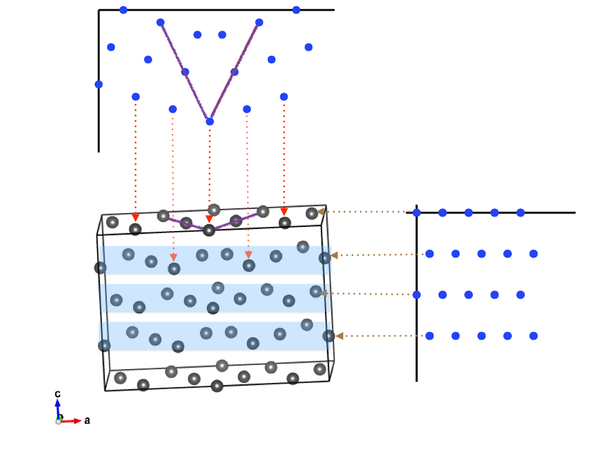
\includegraphics[width=55mm]{vesta_two_dimension.jpeg} 
     \caption{VESTAの投影図を2次元化した図.}
  \label{fig:one}
\end{center}
\end{figure}

\section{各用途に合わせた出力結果}
ソフトを開発していく中で,様々な用途に合わせて原子配列を表示することが可能になった. まず,削除操作を表した原子配列の表示では,図\ref{fig:two}の(a)のように,削除の有無によって原子の色と大きさを変える描画をおこなった.その結果,削除された原子の個数,並びに各位置を視覚的に把握することができた. また,図\ref{fig:two}の(b)のように,構造緩和による原子の移動を三面図で表示した.これにより,原子が移動した経路,並びに構造緩和に過ちが生じていないかを容易に確認することが可能となった. さらに,指定したz軸の層の原子を白抜きする機能を追加したことにより,上面から見た各層の原子の位置を正確に把握できるようになった.

\begin{figure}[h]
\begin{center}
\begin{tabular}{cc}
   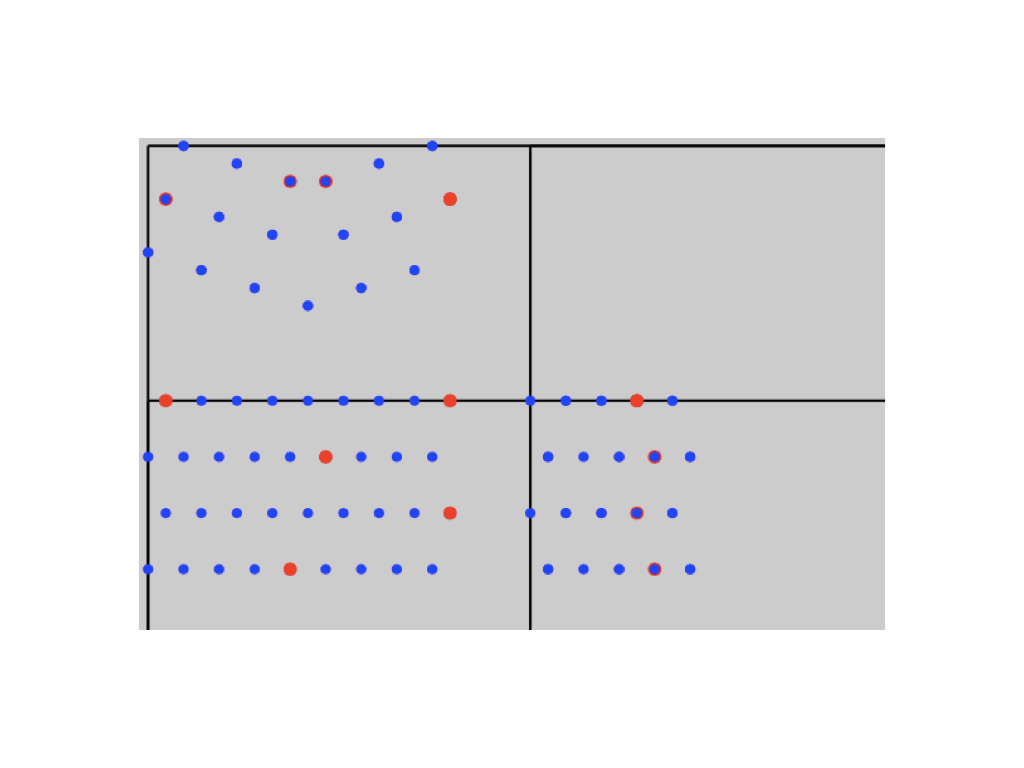
\includegraphics[width=48mm]{deleted_found.jpeg} &
   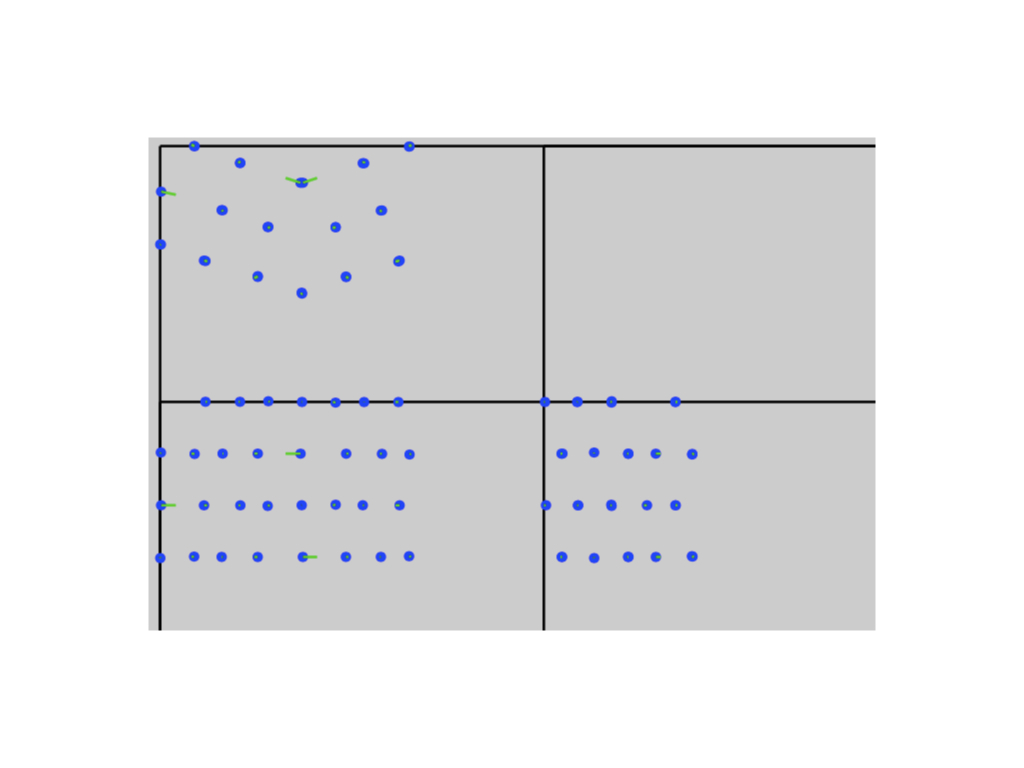
\includegraphics[width=48mm]{change_position.jpeg} \\
   (a) & (b)
\end{tabular}
  \caption{(a) 削除した原子の識別表示と(b)構造緩和による原子移動を表した三面図.}
  \label{fig:two}
\end{center}
\end{figure}


\section{考察}
三面図で原子配列を描画したことにより,構造緩和前後の原子座標を格納したPOSCARファイル内に原子が一つ不足していることを発見できた.したがって,粒界原子配列の構造緩和をおこなう計算を見直していく必要がある.

\begin{thebibliography}{9}
\bibitem{iwasa} 原子削除操作を加えた対称傾角粒界のエネルギー計算, 岩佐 恭佑(関西学院大学 理工学部研究科情報科 学士論文 2016). 
\bibitem{mvc} MVC(Model-View-Controller)を理解する, CakePHP.
\bibitem{three_views} 三面図(機械設計のための基礎製図), 独立行政法人 海上技術安全研究所, NMRI.
\end{thebibliography}

\end{document}
